%%%%%%%%%%%%%%%%%%%%%%%%%%%%%%%%%%%%%%%%%%%%
% Chapitre 3
%%%%%%%%%%%%%%%%%%%%%%%%%%%%%%%%%%%%%%%%%%%%

\chapter{Comparaison de groupes}
\label{Chapter3}

La comparaison de groupes consiste à chercher les changements, statistiquement significatifs, entre deux populations d'observations. 
En imagerie médicale, cela revient dans la plupart des cas d'étude, à comparer une population de sujets atteints d'une pathologie avec une population de sujets sains afin de mettre en avant les zones affectées par la maladie.
Cette méthode mathématique comporte deux parties centrales de traitements : la régression et l'analyse statistique. 
La première permet d'expliquer les observations grâce à des variables explicatives connues et associées à chaque observation, ainsi qu'à des régresseurs à estimer pour chacun des deux groupes.
La deuxième partie sert à tester si ces régresseurs présentent une différence statistiquement significative.
Ces parties sont généralement précédées par des pré-traitements tels que la correction des artefacts d'acquisition, le recalage et le fitrage.\\

% \minitoc

%----------------------------------------------------------------------------------------

\section{Contexte}
La comparaison de groupes s'inscrit dans un contexte de recherche pure. 
Il n'y a aucune application directe du praticien à son patient en clinique.
Par contre, les aboutissements d'une telle méthode apportent au médecin, une meilleure compréhension du mécanisme de la pathologie et une aide au diagnostique et au pronostique.
Les utilisateurs de cette approche sont aussi bien des scientifiques travaillant à résoudre les différents problèmes rencontrés (voir Section \ref{problematiques}) que des médecins analysant les résultats obtenus par des logiciels tels SPM ou SnPM\footnote{\url{http://warwick.ac.uk/snpm}}.

D'un point de vue parenté, cette méthode s'apparente à la comparaison longitudinale de deux images de tenseur consécutives d'un même patient \cite{Grigis2012}.
Le fait de prendre deux populations de sujets plutôt que seulement deux images longitudinales permet de réduire la variabilité inter-individus. 
Comme conséquence, cette approche rend le système statistique plus puissant pour détecter les zones de changements entre les deux groupes et non plus les variations structurelles d'un individu à un autre.

De plus, il est à noter que les cohortes ont des tailles de plus en plus importantes.
Comme exemples de base de données aux échelles nationale et internationale, Baltazar\footnote{\url{https://clinicaltrials.gov/ct2/show/study/NCT01315639?term=baltazar&rank=1}}, ADNI\footnote{\url{http://adni.loni.usc.edu/}} ou encore OSEP\footnote{\url{http://www.ofsep.org/fr/}} peuvent être citées.
La grande taille des échantillons dans un modèle statistique est un atout car cela rend les résultats obtenus plus fiables.


\section{Problématiques}
\label{problematiques}
Dans cette section, les différents problèmes intrinsèques à la comparaison de groupes seront abordés.
Trois axes principaux ont été dégagés et sont exposés dans l'ordre suivant : 
les problématiques liées à la multivariabilité des données, les problématiques provenant de la pré-étape de recalage et
les problématiques dûes à la géométrie du tenseur de diffusion.
Les travaux de cette thèse ont consisté à apporter des réponses ou encore à évaluer l'influence de ces trois points.

\subsubsection*{Problématique liée à la dimension des données}
Ce paragraphe n'est pas un état de l'art. 
Il sert simplement à introduire aux lecteurs les problèmes rencontrés à cause de la dimension des données.
Un état de l'art détaillé est proposé dans la prochaine section (voir \secref{etat_art}).\\
La multi-dimensionnalité des données est le problème majeur des images du tenseur de diffusion autant pour les pré-traitements que pour les traitements. 
Les tenseurs s'expriment sous forme de matrice de dimension 3, symétrique et définie positive, $D \in Sym^{+}(3)$~\cite{Basser1994} :
\begin{center}
    $\textbf{D} = \left[\begin{array}{ccc}
    D_{11} & D_{12} & D_{13}\\
    * & D_{22} & D_{23}\\
    * & * & D_{33}
    \end{array}\right]$
\end{center}
Toutes les informations permettant de décrire globalement la diffusion en un voxel, sont contenus dans cette matrice : 
diffusion radiale et axiale, orientation de la diffusion, diffusion moyenne ou encore fraction d'anisotropie.
Comme expliqué en début de chapitre, la comparaison de groupes consiste en deux opérations mathématiques : la régression et l'analyse statistique.
Elles peuvent être sous-divisées en opérations simples telles que l'addition, la soustraction, la division, la somme, la puissance ...
Ces opérations s'appliquent très facilement sur des scalaires.
Cependant appliquer une de ces opérations sur les images de tenseur de diffusion, revient à faire du calcul matriciel ce qui peut considérablement compliquer la tâche.
De plus, les hypothèses statistiques nécessaires pour la régression et l'analyse statistique peuvent totaltement différer entre le scalaire et la matrice.\\
Plusieurs techniques sont possibles pour traiter ce type de données. 
La première, la plus utilisée, consiste à extraire des scalaires (FA ou MD) de la matrice et à appliquer les méthodes de détection directement sur ces scalaires.
Deuxièment, des méthodes proposent de s'occuper seulement des 6 éléments supérieurs de la matrice en les concatenant dans un vecteur.
\begin{center}
    $vect(\textbf{D}) = \left[\begin{array}{cccccc}
    D_{11} & D_{12} & D_{13} & D_{22} & D_{23} & D_{33}
    \end{array}\right]^{T}$
\end{center}
Troisièment, certaines techniques s'appliquent directement sur la matrice entière du tenseur de diffusion.
%%%%%%%%%%%%%%%%%%%%%%%%%%%%%%%%%%%%%%%%%%%%%%%%%%%%%%%%%%%%%%%%%%%%%%%%%%%%%%%%
\subsubsection*{Problématique liée à la géométrie de l'espace des tenseurs}
Comme expliqué au \chapref{Chapter1}, page \pageref{Chapter1} du manuscrit, un tenseur de diffusion $\textbf{D}$ 
est représenté mathématiquement par une matrice de dimension 3, symétrique et définie positive, $\textbf{D} \in Sym^{+}(3)$~\cite{Basser1994}.
La définition positive du tenseur se vérifie si toutes ses valeurs propres sont strictement positives.
Cette géométrie particulière implique que l'espace du tenseur n'est pas un espace Euclidien mais un cône convexe défini dans cet espace vectoriel. 
Dans ce sous-espace, des métriques de l'espace Euclidien restent stables mais elles n'imposent aucune contrainte sur la positivité des tenseurs.
Certaines opérations entrainent des valeurs propres nulles ou négatives.
Prenons comme exemple simple, le résultat de la différence Euclidienne de deux tenseurs $\textbf{D}_{diff}$. 
Dans tous les cas, la matrice résultat est symétrique $\textbf{D}_{diff} \in Sym(3)$ mais pas forcément définie positive.

Dans ce contexte, plusieurs travaux ont été consacrés au développement de métriques, précédemment définie sur l'espace Euclidien, 
appliqués à un espace non plus \og plat \fg mais \og courbé \fg pour lequel les valeurs propres nulles ou négatives se situent à l'infini. 
Il est question de l'espace Riemannien, souvent représenté par une shpère.
La distance est alors définie, de manière intrinsèque, comme un chemin géodésique entre deux points.
Dans ces précédents travaux~\cite{Pennec1999,Pennec2004,Pennec2006}, Pennec a appliqué les métriques appartenant à des variétés Riemanniennes aux tenseurs de diffusion
permettant de préserver leur nature positive.

\begin{figure}[htpb]
    \centering
    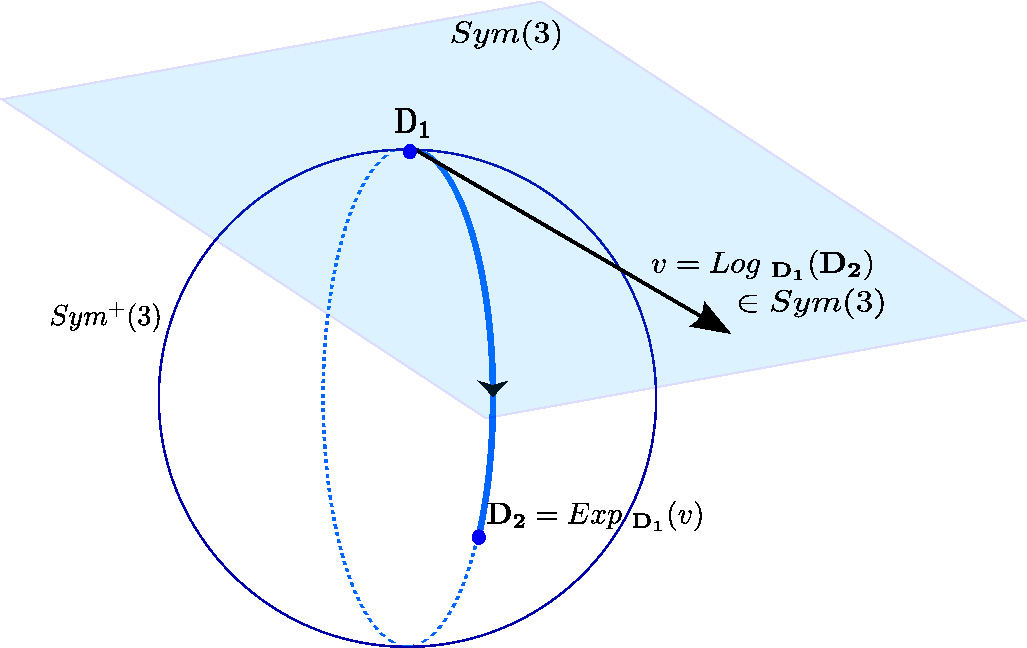
\includegraphics[scale=0.6]{Images/log_exp_map_sphere.pdf}
    \caption{\label{fig_log_exp_map} Illustration des cartes Riemanniennes logarithmique et exponentielle.}
\end{figure}

Cependant, à cause de la courbure de l'espace, l'implémentation de ces méthodes devient plus complexe et le temps d'exécution des calculs est considérablement plus long.
Dans l'optique d'éviter ces contraintes tout en conservant les propriétés théoriques convenables de l'espace Riemannien, 
de nouvelles métriques, appelées Log-Euclidiennes, sont proposées par~\cite{Arsigny2005,Arsigny2006} dans un cadre Riemanien.
Elles permettent de faire des \og aller-retours \fg entre un tenseur $\textbf{D}_\textbf{2}$ appartenant à l'espace des matrices symétriques définies positives $Sym^{+}(3)$ 
et son log-tenseur associé $Log_{\ \textbf{D}_\textbf{1}}(\textbf{D}_\textbf{2})$ de l'espace des matrices symétriques $Sym(3)$,
via le plan tangentiel au tenseur $\textbf{D}_\textbf{1}$ (voir le graphique en \figref{fig_log_exp_map}).
Par conséquent, l'enchainement suivant est rapide d'exécution, simple à implémenter et il garantit que le résultat est bien un tenseur de diffusion.
Le tenseur $\textbf{D}_\textbf{2}$ est projeté sur l'espace vectoriel associé au tenseur $\textbf{D}_\textbf{1}$.
Ensuite les métriques Euclidennes sont appliquées sur le log-tenseur $Log_{\ \textbf{D}_\textbf{1}}(\textbf{D}_\textbf{2})$ et $\textbf{D}_\textbf{1}$.
Enfin, le résultat peut être projeté de nouveau dans l'espace courbé.

Des travaux ont déjà évalué l'impact de telles métriques pour divers problèmes de traitements sur les tenseurs~\cite{Arsigny2006,Pasternak2010},
mais aucun ne précise la plus appropriée à utiliser, particulièrement dans le contexte de la comparaison de groupes.
%%%%%%%%%%%%%%%%%%%%%%%%%%%%%%%%%%%%%%%%%%%%%%%%%%%%%%%%%%%%%%%%%%%%%%%%%%%%%%%%%%%%%
\subsubsection{Problématique liée à l'étape du recalage}
C'est une étape fondamentale des pré-traitements en imagerie médicale. 
La comparaison de groupes nécessite une mise en correspondance spatiale des structures anatomiques afin de présenter les résultats en terme de regions neuro-anatomiques.
Cette étape permet de placer toutes les images des deux populations dans un même espace commun.

Nous pouvons décrire de manière très succincte le processus d'une telle étape.
Une étape de recalage consiste en une estimation du champ de déformations suivie par une application de ce champ aux images et d'une interpolation.
Plusieurs éléments composent la partie estimation de cette technique : des primitives à mettre en correspondance, un critère de similarité $f$, une transformation $t \in T$ ( $T$ étant le domaine des transformations), une méthode d'optimisation et bien évidemment deux images (une image source $I_s$ et une image de référence $I_r$). 

\begin{equation}
    \min_{t \in T} f(I_r, t(I_s) )
    \label{eq_recalage}
\end{equation}

Pour chaque élément de cette liste, il y a des sous-catégories : transformations globales ou locales, critère de similarité mono-modal ou multi-modal, type de primitives utilisées (voxels, surface, centre de gravité ...) ou encore le type de géométrie des transformations (rigide, affine et non-linéaire).
Dans la littérature, de nombreux travaux proposent des états de l'art complets sur l'étude du recalage en imagerie 
médicale~\cite{Noblet_PhD,Klein2009,Sotiras2013,Oliviera2014} dont certains sont plus spécifiques aux image du tenseur de diffusion~\cite{Zhang2007,Wang2011,Schwarz2014}.
Notre bibliographie s'est orientée autour de techniques de recalage sans structure particulière utilisant tous les voxels de nos images.
% image d'un pipeline 

Deux problématiques liées à l'étape du recalage appliqué aux images de tenseurs de diffusion se dégagent : l'interpolation et la ré-orientation des tenseurs.
En effet, dans le contexte du ITD, l'application d'un champ de transformations peut rencontrer de nombreuses difficultés, notamment dûes à la nature du tenseur de diffusion.\\

Premièrement, l'interpolation de deux tenseurs n'est pas évidente. 
Une interpolation linéaire de deux tenseurs avec une métrique Euclidienne de forme identique mais d'orientation perpendiculaire, 
un vertical et l'autre horizontal, produit une shpére et non pas un tenseur orienté à 45 degrés.
Ce problème rejoint celui présenté ci-dessus avec le paragraphe sur \og Problématique liée à la géométrie de l'espace des tenseurs \fg.
La \figref{fig_interpolation} illustre une interpolation linéaire des tenseurs avec trois métriques, une de chaque géométrie.\\
\begin{figure}[htpb]
    \centering
    \includegraphics[scale=0.8]{Images/interpolation_arsigny.pdf}
    \caption{\label{fig_interpolation} Illustration~\cite{Arsigny2005} d'interpolation linéaire des tenseurs avec des métriques différentes. \textbf{Haut} : métriques Euclidenne, \textbf{Milieu} : métrique Riemannienne. \textbf{Bas} : métrique Log-Euclidienne}
\end{figure}

Deuxièment, l'orientation des tenseurs après l'application de la transformation estimée peut se révéler particulièrement contraignante.
Dans l'image source transformée, les voxels prennent, par tranformée inverse, les tenseurs présents dans l'image source avant recalage.
Ces tenseurs ont une décomposition spectrale qui permet d'obtenir les axes de l'ellipsoïde ($\overset{\rightarrow}{e_1}$, $\overset{\rightarrow}{e_2}$, $\overset{\rightarrow}{e_3}$) 
et les valeurs propres associées ($\lambda_1$, $\lambda_2$, $\lambda_3$).
Cette décompostion n'a pas pris en compte les tranformations subies par l'image.
Ainsi dans l'image source tranformée, les tenseurs auront les même décompositions spectrales et par conséquent, les même orientations.
Prenons comme exemple de tranformation, illustré par la \figref{fig_reorientation}, un simple rotation de 45 degrés.
L'image (a) représente l'image source de base.
L'image (b) montre l'image (a) ayant subie une rotation de 45 degrés. 
Il est visible que les tenseurs n'ont pas suivi la rotation et reste tels qu'ils sont dans l'image (a).\\

\begin{figure}[htpb]
    \centering
    \includegraphics[scale=0.6]{Images/reorientation.pdf}
    \caption{\label{fig_reorientation} Illustration simple du problème de ré-orientation des tenseurs : rotation d'une image de tenseurs de diffusion de 45 degrés. (a) image d'origine, (b) image après application du champ de transformation,
    (c) image après application du champ de transformation et ré-orientation}
\end{figure}


\section{État de l'art en imagerie du tenseur de diffusion}
\label{etat_art}
En premier lieu, nous précisons que cet état de l'art ne s'intéresse qu'aux méthodes de détection de changements spécifiques
à l'imagerie du tenseur de diffusion et à la comparaison de groupes.
De nombreux articles et doctorats portent sur la détection de changements dans les divers autres domaines.
Pour une liste plus générale des références bibliographiques sur la détection de changements en imagerie de diffusion 
se réferrer au manuscrit de thèse d'Antoine Grigis \cite{Grigis_PhD}.\\

Les méthodes de détection peuvent être classées en trois grandes familles : 
les méthodes utilisant les indices scalaires dérivés du tenseur (FA ou MD), 
celles basées sur les vecteurs déduit du tenseur $vect(\mathbf{D})$
et enfin celles prenant en compte toute la matrice du tenseur $\mathbf{D}$.

La famille la plus grande est celle des méthodes basées sur les indices scalaires.
En effet, ces méthodes ne souffrent pas de problèmes de multi-dimensionnalité, ni de problèmes de variétés (voir \secref{problematiques}) : 
les indices scalaires commes leur nom l'indique sont des scalaires définis sur le domaine Euclidien.\\



Des modèles utilisant la matrice entière du tenseur ont aussi été développées \cite{Zhu2009, Schwartzman2010, Yuan2012, Bouchon2014, Kim2014} 
mais elles doivent faire face à l'incapacité du cadre euclidien pour tenir compte de la définie-positivité d'un tenseur de diffusion.\\

Comme expliqué dans la \secref{problematiques}, deux variétés avec des métriques prenant en compte la définie-positivité des tenseurs ont été proposées :
le Log-Euclidien \cite{Arsigny2006} et le domaine Riemanien \cite{Pennec1999}.\\

Quelques travaux ont déjà évalué l'impact des différentes métriques (Euclidiennes, Log-Euclidennes et Riemmaniennes) 
pour divers problèmes de traitement d'image \cite{Arsigny2006, Pasternak2010}, 
mais il n'y a toujours pas de consensus sur la variété la plus appropriée pour le traitement des tenseurs de diffusion, 
en particulier dans le contexte de comparaison de groupes.



\section{Pré-traitements}
\label{sec:preprocessing}
Cette section présente les trois pré-traitements implémentés dans la chaine de traitements : 
la correction des artefacts liés à l'acquisition,  l'estimation des tenseurs, le recalage qui permet de placer tous les sujets dans un même référentiel anatomique 
et enfin l'étape de filtrage permettant de lisser les observations afin de réduire le bruit et ainsi à améliorer les détections statistiques.

\subsection{Corrections des artefacts d'acquisition}
L'IRM de diffusion permet d'acquérir une série d'images pondérées en diffusion (DWI)
à partir de laquelle est estimée l'image du tenseur de diffusion (ITD).
Lors de l'acquisition, des artéfacts peuvent apparaître 
ce qui peut entraîner des distorsions importantes et compromettre les résultats des études.
Ils sont référencés dans la revue \cite{Jones2010}.
La plupart sont corrigés lors des pré-traitements afin d'obtenir des données 
les plus fiables possibles pour les analyses statistiques.
Pour cela, nous avons utilisé la méthode \og eddy\_current \fg de la librairie FSL\footnote{\url{http://fsl.fmrib.ox.ac.uk/fsl/}}.
% De plus, habituellement les gradients de diffusion sont normalisés mais nous avons eu un cas où ce n'était pas le cas. Nous avons alors dû corriger cette erreur et par défaut nous avons inclus une normalisation dans notre chaine de traitements. Cette opération par défaut est importante même si elle n'est que peu de fois exécutée car il suffit d'une série d'image avec des gradients de diffusion non normalisés pour fausser les résultats de la chaine de traitement.

\subsection{Estimation pondérée des tenseurs de diffusion}
La méthode classique d'estimation des tenseurs est celle des \og moindres carrés \fg.
Elle, ainsi que ses limites, sont décrites plus tôt dans le manuscrit (voir \chapref{Chapter1}).
Dans notre chaine de traitements, nous avons opté pour une méthode pondérée des moindres carrées proposé par \cite{Zhu2007} car
elle tient compte du fait que le bruit est un mélange de plusieurs bruits distribués différemment.
Les $n$ mesures pondérées en diffusion pour chaque voxel s'exprime sous la forme d'un triplet $(S_i, r_i, b_i)$ pour $i=1\ldots n$.
L'équation du signal acquis, et par conséquent bruité, s'écrit de la manière suivante après une transformée logarithmique pour linéariser le signal exponentiel : 
\begin{center}
    $log(S_i) = log(S_0) - b_i\textbf{r}_\textbf{i}^T\textbf{D}\textbf{r}_\textbf{i} + \eta_i$
\end{center}
Avec $S_i$ la $i^\text{ème}$ image pondérées en diffusion, $S_0$ l'image sans pondération, $b_i$ la b-valeur correspondante,
$\textbf{r}_\textbf{i} = (r_{i,1}, r_{i,2}, r_{i,3})^T$ le $i^\text{ème}$ vecteur de gradient de diffusion, $\eta_i$ le bruit lié à l'aquisition 
et enfin $\textbf{D}$ le tenseur de diffusion.
La méthode impose aux gradients de diffusion d'être distribués sur la sphère unité. 
Cela requière une normalisation au préalable des $n$ directions des gradients de diffusion pour qu'ils remplissent la condition suivante :
$\textbf{r}_\textbf{i}^{T}\textbf{r}_\textbf{i} = 1$.
L'estimation est initialisée par une méthode des moindres carrés classique suivie par plusieurs itérations $k_0 = 1\ldots 5$ d'une estimation par les moindres carrés pondérés.
Cette méthode est efficace et rapide d'autant plus que, comme démontré dans l'article \cite{Zhu2007}, 
une seule itération suffit lorsque le nombre de gradients de diffusion est égal ou supérieur à 30.
L'algorithme est détaillé ci-dessous par \algoref{algo:estimation_tenseur_2}.

\begin{center}
    \begin{minipage}[c]{0.9\textwidth}
	\begin{algorithm}[H]
	    \vspace*{0.5em}
	    \Data{
		$log(S_i) = z_i^T\theta + exp(-z_i^T\theta)\sigma\epsilon_i$ avec
		$z_i^T = (1, -b_i(r_{i,1}^2, 2r_{i,1}r_{i,2}, 2r_{i,1}r_{i,3}, r_{i,2}^2, 2r_{i,2}r_{i,3}, r_{i,3}^2))$
		et $\theta = (log(S_0), D_{11}, D_{12}, D_{13}, D_{22}, D_{23}, D_{33})$}\vspace*{1em}		
	    \Res{Estimation des 7 paramètres de $\theta$ : $\theta^{(k_0)} = (log(S_0), D_{11}, D_{12}, D_{13}, D_{22}, D_{23}, D_{33})$}
	    \Deb{
		initialisation $k = 0$ : $\hat{\theta}^{(k)} = ( \sum_{i=1}^{n} z_i z_i^T )^{-1} \sum_{i=1}^{n} z_i\ log(S_i)$\;\vspace*{1em}
		\Pour{$k_0$ itérations}{
		    $w_i^{(k)} = exp(2z_i^T\hat{\theta}^{(k)})$\;\vspace*{1em}
		    $\hat{\theta}^{(k+1)} = (\sum_{i=1}^{n} w_i^{(k)}z_iz_i^T)^{(-1)} \sum_{i=1}^{n} w_i^{(k)}z_i\ log(S_i)$\;
		}
	    }\vspace*{0.5em}
	    \caption{\label{algo:estimation_tenseur_2}Estimation du tenseur de diffusion par les moindres carrés pondérés}
	\end{algorithm}
    \end{minipage}
\end{center}

Pour mesurer la différence entre les méthodes des moindres carrées classiques et des moindres carrées pondérées, 
nous avons simulé un jeu de données de diffusion (type DWI) de synthèse basé sur les simulations introduites par \cite{Zhu2007} dans la section 3.1 de son article.
Nous avons effectué les deux estimations pour différentes valeurs du rapport signal sur bruit.
Pour chaque méthode, nous avons calculé l'erreur quadratique moyenne entre l'image de tenseurs d'origine et l'image de tenseurs estimée.
Nous avons mesuré une réduction d'erreur de 9\% en utilisant cette méthode comparée avec un moindres carrés classique.\\
{\color{red}ILLUSTRATIONS}

\subsection{Recalage}
L'état de l'art sur le sujet du recalage est disponible dans la \secref{problematiques} présentant les problématiques \ref{problematiques} en page \pageref{problematiques}.
Dans ce paragraphe, les trois méthodes de recalage utilisées dans la thèse seront exposés, ainsi que les raisons qui nous ont poussés à ces choix en particulier. 
Au cours de la thèse, nous nous sommes intéressé à l'influence que le recalage peut avoir sur les résultats des méthodes de détection. 
Et notamment aux fausses détections que peuvent engendrer une mauvaise ré-orientation ou une mauvaise estimation des déformations.
Pour répondre à la problèmatique présentée, nous avons sélectionné deux type des recalage différents : 
un recalage basé sur les cartes de scalaire avec une ré-orientation des tenseurs après l'application du champ de déformations 
et un recalage basé sur les cartes de tenseurs avec une ré-orientation des tenseurs directement intégrée de manière analytique dans la fonction de coût.

\subsubsection*{Recalage sur les images de FA}
La première méthode~\cite{Noblet2006} appartient au type de techniques le plus utilisée par la communauté en comparaison de groupes pour le ITD : 
les recalages qui estiment les champs de déformations sur les cartes de fraction d'anisotropie (FA) dérivées des images de tenseurs.

Cette méthode fonctionne en deux étapes.
Dans un premier temps, elle va estimer les transformations par la méthode des moindres carrées en se basant sur l'information mutuelle des images de FA.
Puis, dans un deuxième temps, sachant qu'il reste de petites distorsions anatomiques entre les images, 
un second recalage plus raffiné est effectué à l'aide d'une méthode non-rigide 
qui va estimer un modèle de déformation paramétrique multi-échelles toujours basé sur l'information mutuelle.
Ce recalage déformable peut être très puissant et compenser toutes les différences, de type anatomique ou pathologique, entre les images.
Pour éviter cela,~\cite{Noblet2006} propose d'imposer une contrainte de préservation de la topologie ainsi qu'un terme de régularisation.

Une fois les transformations finales estimées, elles sont appliquées sur les images de tenseurs en utilisant la méthode de 
Préservation de la Direction Principale~\cite{Alexander2001} pour ré-orienter les tenseurs correctement.

\subsubsection*{Recalage sur les images de tenseurs}
La deuxième technique appartient à la nouvelle génération qui estime les transformations directement sur les images de tenseurs.
Le défi du recalage d'images de tenseurs de diffusion est la multi-dimension des données et leur ré-orientation lors de l'application des transformations.
Une analyse comparative complète sur les différences entre 6 recalages basés scalaire et 2 basés tenseurs sont présentés par~\cite{Wang2011}.
Dans leur étude, la méthode \dtitk~\cite{Zhang2006, Zhang2007, Keihaninejad2013} montre les meilleurs résultats d'après les trois critères d'évaluation qu'ils proposent.
Les auteurs concluent en recommandant l'algorithme \dtitk par rapport aux autres méthodes déformables basées sur les tenseurs.
Cet outils de recalage est disponible en ligne\footnote{\url{http://www.nitrc.org/projects/dtitk}}.\\

La méthode \dtitk permet d'estimer les 12 paramètres d'une transformation affine $\textbf{p}$.
Cette estimation est faite morceau par morceau ce qui rend le champ des transformations globales non-linéaire.
L'expression de la transformation affine $F$ est décomposée en 3 matrices de base appliquées au voxel $x$ : 
\begin{equation}
    F(x) = (QS)x + T
    \label{fct_affine_dtitk}
\end{equation}
avec $T$ une matrice de translation, $S$ une matrice de pure déformation et $Q$ une matrice de pure rotation.
L'application de cette matrice $Q$ permet de ré-orienter un tenseur $\textbf{D}$ : $Q\textbf{D}Q^t$~\cite{Alexander2001}.
La méthode définit une fonction de coût $O$ qui intègre de façon explicite cette ré-orientation des tenseurs dans son expression :
\begin{equation}
    O(\textbf{p}) = \int_{\mathcal{R}^3} \|\textbf{D}_s((QS)x + T) - Q\textbf{D}_rQ^t\|^2dx
    \label{fct_cout_dtitk}
\end{equation}
avec $\textbf{D}_r$ et $\textbf{D}_s$ respectivement le tenseur de référence et le tenseur source à déformer.\\

De plus, la méthode \dtitk estime les 12 paramètres $\textbf{p}$ de la transformation affine morceau par morceau sur des régions de taille égale $\Omega_i$
en imposant une contrainte de continuité inter-régions.
Pour cela, l'algorithme essaie de minimiser la différence entre les transformations affines de deux régions.
\begin{equation}
    \int_{\Omega_i\bigcap\Omega_j} \|F_i(x) - F_j(x)\|dx
    \label{fct_cont_dtitk}
\end{equation}
L'expression analytique des équations \eqref{fct_cout_dtitk},\eqref{fct_cont_dtitk} permet une résolution du problème par les gradients conjugués.\\

\begin{figure}[htpb]
    \centering
    \includegraphics[scale=0.7]{Images/dtitk_hierarchie.pdf}
    \caption{\label{fig_dtitk_hierarchie}Illustration de l'approche hiérarchique de l'algorithme \dtitk.
    (a) est la représentation du partage initial ($n=2$) grossier de l'image avec les estimations des transformations sur chaque région.
    (b) est la représentation au niveau supérieur ($n=4$) avec l'estimation des transformations initialisée par les transformations du niveau inférieur.}
\end{figure}
Les transformations finales sont estimées par une approche hiérarchique illustrée par la \figref{fig_dtitk_hierarchie}.
L'algorithme estime les premières transformations $F_i^{n}$ sur une image découpée grossièrement ($n=4$ régions sur chaque côté de l'image 3D).
Par la suite, il raffine son estimation en partageant plus finement l'image ($n=8, 16$) et en initialisant les transformations avec celles du niveau inférieures.

\subsubsection*{Recalage sur les images d'IRM de T1}
Dans son article, \cite{Tustison2014} met en avant un fait important :
estimer les tranformations du recalage sur les même cartes de données sur lesquelles l'analyse statistique
sera effectuée, revient à introduire un biais dans le modèle favorisant les détections.
Il appelle ce phénomène, \og circularity bias \fg et cela se traduit pas une augmentation générale des p-valeurs.
Pour supprimer ce biais, \cite{Tustison2014} conseille d'éviter les recalage basés sur le même jeu de données 
que celui utilisé pour l'analyse statistique lors de la compraison de groupes.
À la place, un recalage en deux étapes est recommandé. 
Dans un premier temps, un recalage multi-modal et intra-individu est effectué entre les cartes de FA vers les cartes d'IRM de T1.
Il est suivi, dans un deuxième temps, par un recalage sur les cartes T1 inter-individus combinant une méthode affine et une méthode non-linéaire~\cite{Noblet2006}.


\subsection{Filtrage}


Après l'étape de recalage, il est recommandé d'utiliser un filtre sur les images de tenseurs dans le but de lisser les observations, de réduire le bruit présent et ainsi contribuer à améliorer les détections statistiques.
